\chapter{Pendahuluan}

\section{Latar Belakang}

KIRI (\url{http://kiri.travel}, gambar \ref{fig:1_kiri}) adalah sebuah situs yang dikelola oleh PT. Kirana Sistem Transportasi, yang menyediakan layanan navigasi dari satu titik ke titik lain dengan memanfaatkan transportasi publik. Layanan ini diberikan secara gratis kepada pengunjung situs / pengguna aplikasi bergerak mereka. Untuk mendukung layanan tersebut, tim KIRI melakukan kurasi rute angkot secara mandiri di Bandung dengan mencatat perjalanan setiap trayek menggunakan peralatan GPS (\textit{Global Positioning System}). Pada perkembangannya, KIRI melakukan ekspansi ke beberapa kota lainnya termasuk Jakarta. Hanya saja, karena keterbatasan sumberdaya, data di Jakarta dimasukkan hanya berbekal data yang tersedia di internet tanpa validasi di lapangan. Di sisi lain, ada beberapa pihak yang tertarik akan layanan KIRI di Bandung dan berniat untuk mendapatkan layanan serupa di kota mereka.

\begin{figure}
	\centering
	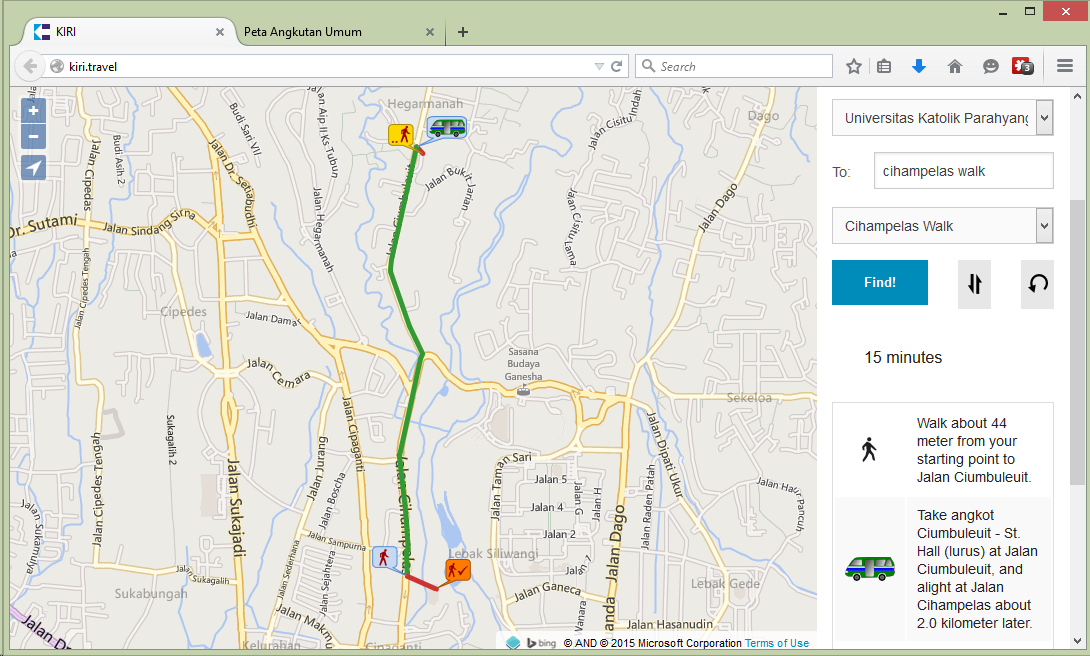
\includegraphics[scale=0.5]{Gambar/1_kiri}
	\caption{Situs Web KIRI} 
	\label{fig:1_kiri}
\end{figure}

Situs Peta Angkutan Umum (\url{https://angkot.web.id}, gambar \ref{fig:1_angkotwebid}) merupakan sebuah situs yang dikembangkan oleh Fajran Iman Rusadi. Situs ini memungkinkan pengguna publik untuk melihat, memasukkan, atau memperbaiki data rute angkot di Indonesia (dengan kata lain, \textit{crowdsourcing}). Seperti KIRI, layanan ini juga diberikan secara gratis.

\begin{figure}
	\centering
	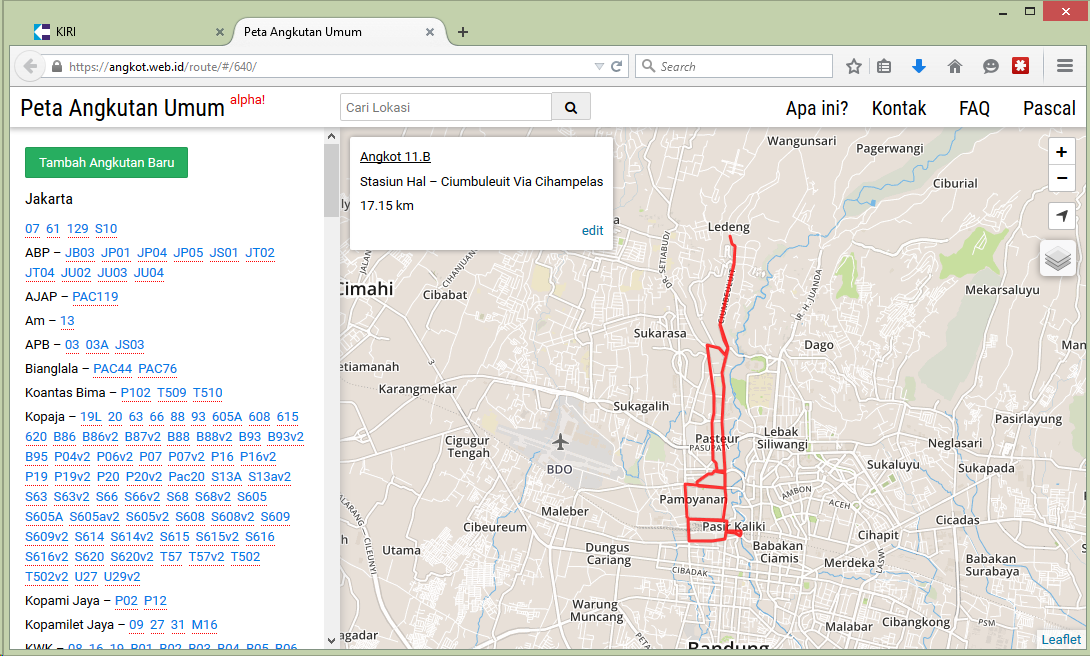
\includegraphics[scale=0.5]{Gambar/1_angkotwebid}
	\caption{Situs Web Peta Angkutan Umum}
	\label{fig:1_angkotwebid}
\end{figure}

Sebagai situs navigasi, KIRI membutuhkan data yang akurat. Di sisi lain, situs Peta Angkutan Umum membuka kesempatan bagi penggunanya untuk berkontribusi memperbaiki rute yang kurang akurat. Oleh karena itu, integrasi antara kedua situs ini akan memberikan nilai tambah bagi keduanya. Di satu sisi, KIRI akan dapat menghasilkan rute yang lebih akurat. Di sisi lain, situs Peta Angkutan Umum pun akan lebih hidup karena bantuan publikasi dari KIRI.

\section{Rumusan Masalah}

Dari latar belakang yang sudah dijelaskan, peneliti bermaksud untuk mengintegrasikan data yang dimiliki kedua situs web tersebut. Integrasi tersebut dirumuskan ke dalam masalah-masalah berikut:

\begin{enumerate}
	\item Bagaimana mekanisme penarikan data oleh KIRI terhadap Peta Angkutan Umum secara otomatis?
	\item Bagaimana menyimpan data yang digunakan, terutama untuk mendukung pemisahan antara data yang dimiliki oleh KIRI sendiri dengan data yang ditarik dari Peta Angkutan Umum?
	\item Bagaimana merancang protokol yang optimal, sehingga kebutuhan \textit{bandwidth} dapat dihemat?
	\item Bagaimana respon pengguna KIRI terhadap fitur yang diimplementasikan?
\end{enumerate}

\section{Tujuan}

Berdasarkan rumusan masalah yang sudah dijabarkan, maka didefinisikan tujuan-tujuan berikut:

\begin{enumerate}
	\item Merancang dan mengimplementasikan mekanisme penarikan data otomatis oleh KIRI terhadap Peta Angkutan Umum.
	\item Merancang dan mengimplementasikan penyimpanan data, sehingga mendukung pemisahan data antara rute milik KIRI dengan data yang ditarik dari Peta Angkutan Umum.
	\item Merancang dan Mengoptimasi protokol komunikasi yang digunakan, sehingga kebutuhan \textit{bandwidth} dapat dihemat.
	\item Mempelajari respon pengguna publik  KIRI terhadap fitur yang diimplementasikan.
\end{enumerate}

\section{Batasan Masalah}

Penelitian ini memiliki batasan-batasan seperti berikut:

\begin{enumerate}
	\item Penelitian dilakukan untuk rute angkot kota Bandung saja.
	\item Dengan alasan kerahasiaan, penelitian ini tidak membahas keseluruhan bagian dari KIRI dan Peta Angkutan Umum, melainkan hanya bagian yang terkait penelitian saja.
\end{enumerate}

\section{Metode Penelitian}

Dalam penelitian ini, akan dilakukan langkah-langkah berikut:

\begin{enumerate}
	\item Melakukan studi terhadap mesin navigasi KIRI, protokol Peta Angkutan Umum, serta teori-teori lain yang mendukung kedua hal tersebut.
	\item Melakukan analisis untuk menemukan hal yang dapat dilakukan untuk mengintegrasikan data kedua situs tersebut.
	\item Melakukan perancangan untuk implementasi integrasi kedua sistem tersebut.
	\item Melakukan implementasi dari rancangan yang sudah dilakukan.
	\item Melakukan publikasi terhadap pengguna publik KIRI sehingga pengguna dapat menguji hasil implementasi tersebut.
	\item Menganalisa dan menarik kesimpulan atas hasil penelitian yang telah dilaksanakan.
\end{enumerate}

\section{Sistematika Penulisan}

Berikut adalah sistematika penulisan dari dokumen ini:

\begin{itemize}
	\item Bab 1 membahas latar belakang, rumusan masalah, tujuan penulisan, batasan-batasan, serta metode yang digunakan pada penelitian ini.
	\item Bab 2 membahas teori-teori yang digunakan dalam penelitian ini, yaitu JSON dan GeoJSON.
	\item Bab 3 menganalisis sistem kini, beserta perubahan-perubahan yang harus dilakukan, mencakup mesin navigasi KIRI, protokol komunikasi, dan optimasi.
	\item Bab 4 membahas perancangan yang dilakukan sebelum mengimplementasikan integrasi yang dimaksud, mencakup mesin navigasi KIRI, protokol, basisdata, beserta antarmukanya.
	\item Bab 5 membahas implementasi serta pengujian dari integrasi yang telah dilakukan.
	\item Bab 6 membahas kesimpulan dari keseluruhan penelitian ini, serta saran-saran yang dapat diberikan untuk penelitian berikutnya.
\end{itemize}